% Brian Mc George
% MCGBRI004
% 13/04/2015

\documentclass[]{article}
\title{Functional Programming Assignment 1\\Theoretical Questions}
\date{13-04-2015}
\author{Brian Mc George\\MCGRBRI004
}
\usepackage{graphicx}
\usepackage{amsfonts}
\usepackage{amsmath}
\usepackage{float}
\usepackage{tabularx}\begin{document}

\maketitle
\newpage

\section{How many non-distrinct states can be generated in \(n\) moves (Question 2.2)?}
The Rubik's cube can be twisted in six directions. For each state, six new (non-distinct) states can be generated. The states generated from \(n\) moves can be represented by the following mathematical function:
\begin{equation}\label{func_states}	
	f(n)=6^n\text{ for all }n \in\mathbb{N}
\end{equation}

\section{Investigate processing speed and memory usage for different values of \(n\) (Question 3.2)}
\subsection{Test System}
The tests were run on an Intel Core i7 2600 (3.4Ghz) processor running Windows 8.1 x64 using the gambit interpreter (v 4.7.4).

\subsection{Effect of \(n\) On Completion Time}
\subsubsection{Testing Methodology}
Tests were conducted for \(n\) up to size 8.
The following function was used to test completion time and memory allocation\begin{equation*}\begin{split}
cubeSolve(rotationString) = \text{(time (solveCube solvedStates (rotate }rotationString \\\text{ '((1 1) (2 1) (3 1) (4 1) (5 3) (6 3) (7 3) (8 3))) 0))}
\end{split}\end{equation*}
The rotation string used for \(n = 8\) was "xyzXYZxy", for \(n = 7\) was "xyzXYZx" etc.\newline\newline The memory allocated would appear to be the memory allocated during the runtime not the total memory used at a particular time. To get faster completion time a non-tail recursive genStates method was used. Two implementations of genStates were written (\textit{genStatesTailRecursive} \& \textit{genStates}), one was tail recursive (completed slower) and the other was not tail recursive (completed faster). For comparison at a size \(n = 7\), solveCube with non-tail recursive genStates completed in 15 seconds with a peak memory usage of 586 MB. The solveCube with tail recursive genStates completed in 240 seconds with a peak memory usage of 273 MB. The non-tail recursive genStates was selected since the assignment brief outlined that it should be able to solve cubes of 7 moves or less. The memory usage only becomes a concern from at least 8 moves.
\subsubsection{Results Obtained}
\begin{table}[H]
\begin{center}
	\begin{tabular}{|r|c|l|}
		\hline
		Size of \(n\)&Memory Allocated (MB)&Completion Time (Seconds)\\
		\hline
		1&0.07728&\textless\space0.001\\
		2&0.556592&0.002\\
		3&3.48304&0.012\\
		4&21.130368&0.070\\
		5&128.346848&0.448\\
		6&786.701024&2.558\\
		7&4824.05504&15.853\\
		8&29659.645296&95.583\\
		\hline
		
	\end{tabular}\caption{Memory usage and completion time for different size of \(n\)}\end{center}
	\label{table:mem_usage}
\end{table}

 The results would indicate an exponential increase in running time and memory usage. The increase in completion time could be as a result of the exponentially increasing search space to find the solution from. The increase in memory usage could be a result of it not being tail recursive as well as the search space, whose size is proportional to \(n\), that needs to be stored. 
 
 \subsection{Memory Usage During Runtime}
 \subsubsection{Testing Methodology}
 The \(cubeSolve\) function defined above was used with the \(rotationString\) for \(n = 7\). Process Explorer was used to track the memory usage during program execution. 
 \subsubsection{Results Obtained}
 
 % Memory Usage Image
 \begin{figure}[H]
 	\centering
 	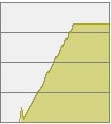
\includegraphics[width=0.2\linewidth]{mem_usage2.jpg}
 	\caption{Memory Usage Over Time (Non-Tail Recursive genStates)}
 	\label{fig:memory_usage}
 \end{figure}
 
  \begin{figure}[H]
  	\centering
  	\noindent\makebox[\textwidth]{
  	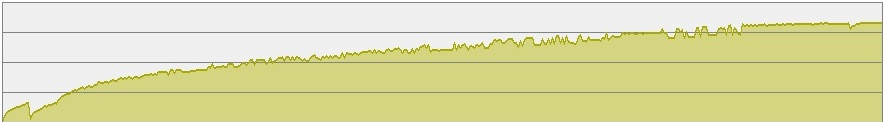
\includegraphics[width=1.2\linewidth]{mem_usage3.jpg}
  }
  	\caption{Memory Usage Over Time (Tail Recursive genStates)}
  	\label{fig:memory_usageTail}
  \end{figure}

 Figure \ref{fig:memory_usage} shows a linear increase in memory usage as the program executes. Figure \ref{fig:memory_usageTail} shows a logarithmic increase in memory usage as the program executes. The tail recursive genStates had a peak memory usage of 273 MB where the non-tail recursive genStates had a peak memory usage of 586 MB. It follows that the tail recursive genStates is more memory efficient than the non-tail recursive genStates. The length of the graph indicates that the solveCube using tail recursive genStates is much slower than than using the non-tail recursive genState. 

\section{Optimise algorithm and calculate reduction in number of states (Question 4)}
\subsection{Optimised function}							
Function \ref{func_states} can be optimised such that from a given state, the new states generated are only those that will not undo the last move.
\begin{equation}
\begin{split}
g(n) =
\begin{cases}
	1 & \text{if }n \in T = \{0\}\\
	6 \times 5^{n-1} & \text{if }n \in \mathbb{N} \setminus T\\
	0 & \text{otherwise}
\end{cases}
\end{split}
\label{fun:func_states_optimised}
\end{equation}
\subsection{Number of states for \(n = 10\)}
\subsubsection{Sum of consecutive powers formula}
The comparison assumes worse case scenario where \textit{solveCube} has to generate maximum number of states, from \(n = 0\) to \(n = 10\) (assumes a new state is generated for \(n = 0\)).
\\\\The sum of consecutive powers formula is used to calculate the sum a number \(x\) up to the power \(n\): 
\begin{equation}
\sum_{i=0}^{n}x^i = \frac{x^{i+1} - 1}{x - 1} \\
\label{eq:sumStates}
\end{equation}
\subsubsection{Six possible moves per rotation}
Using function \ref{eq:sumStates}, the number of states generated by \(solveCube\) for \(n = 10\) can be calculated as follows (where function \ref{func_states} is substituted for \(x^i\)):
\begin{equation*}
\begin{split}
\sum_{i=0}^{10}6^i & = \frac{6^{10+1} - 1}{6 - 1} \\
& = \frac{6^{11} - 1}{5} \\
& = 72559411\text{ states}
\end{split}
\end{equation*}
\subsubsection{No undo moves per rotation}	
Similarly, to calculate the number of states the optimised \textit{solveCube} will generate for \(n = 10\), substitute function \ref{fun:func_states_optimised} for \(x^i\) and adding 1 for the 0 state.
\begin{equation*}
\begin{split}
 1 + \sum_{i=1}^{10} 6 \times 5^{i-1} & = 1 +  (6 \times \sum_{i=1}^{10} 5^{i-1})\\	
 & = 1 +  (6 \times \frac{5^{(10-1)+1} - 1}{5 - 1})\\
 & = 1 +  (6 \times \frac{5^{10} - 1}{4})\\
 & = 14648437 \text{ states} 
\end{split}
\end{equation*}
It follows that the optimised \textit{solveCube} produces 57910974 (79.81\%) fewer states than the unoptimised \textit{solveCube} for \(n = 10\).
\subsection{Results Of Optimisation}
\begin{table}[H]
	\begin{center}
		\noindent\makebox[\textwidth]{%
		\begin{tabular}{|r|c|c|c|c|}
			\hline
			Size of \(n\)&Memory Allocated (MB) &Memory Reduction (\%)&Completion Time (Seconds)& Completion Time Reduction (\%)\\
			\hline
			1&0.077504&-0.29&\textless\space0.001&0\\
			2&0.530832&4.63&0.002&0\\
			3&2.895664&16.86&0.09&25.00\\
			4&14.866848&29.64&0.046&34.29\\
			5&75.620656&41.08&0.251&43.97\\
			6&382.531696&51.38&1.299&49.22\\
			7&1945.344192&59.67&6.336&60.03\\
			8&10000.118816&66.28&31.641&66.90\\
			\hline
			
		\end{tabular}}\caption{Memory usage and completion time for different size of \(n\)}\end{center}
	\label{table:mem_usage}
\end{table}
\section{Discussion on why the non-tail recursive genStates was faster}
Please note this section is based on opinion and not fact. There are a number of possible reasons why the tail recursive genStates behaved slower than the non-tail recursive implementation:
\begin{enumerate}
	\item \textit{The tail recursive implementation was badly written and unoptimised?}\\This is a possibility although other students have also gotten similar slow speeds for theirs too.
	\item \textit{Large number of list copies} \\ This would appear to be the most likely culprit that every time we re-call the function to build up the list it is having to make a copy of the list. Since there are a large number of states the number of times it would have to do a copy could be large.
	\item \textit{Large number of append calls}\\ As far as I am aware the append function is O(N), therefore calling it every recursive call could become costly.
\end{enumerate}
The non-tail recursive genStates builds up the lists separately for each axis, as a result the lists it is handles remain smaller and this may give it faster performance at the cost of some additional memory usage.
\section{Conclusions}
\subsection{Brute force infeasible for large \(n\)}
 Both of the methods shown, tail recursive and non tail recursive, suffer the same issue - exponential computational complexity. The memory and time completion for both expand at a rate that makes both algorithms infeasible for \(n>10\). An algorithm with a smaller computational complexity is required to solve for any large number of rotations.
\subsection{Major improvement when ignoring undo moves}
Ignoring rotations that will undo last move dramatically reduces the number of states that have to be generated at \(n = 10\). For \(n = 8\) a 66.9\% reduction in completion time was obtained. It is a big performance improvement for relatively little work.
\end{document}
